
\chapter{Installation Guide}

\section{Introduction}

The CHOReOS \ee\ (EE) provides a Platform as a Service (PaaS) that automates the distributed deployment of service choreographies in cloud environments. This chapter is targeted mainly to EE \emph{administrators}, providing instructions about how to install, configure, and run the \ee.

We will describe now each one of the components running on the \ee execution environment. They are depicted in Fig.~\ref{fig:ee_components}. 

\begin{figure}
\centering
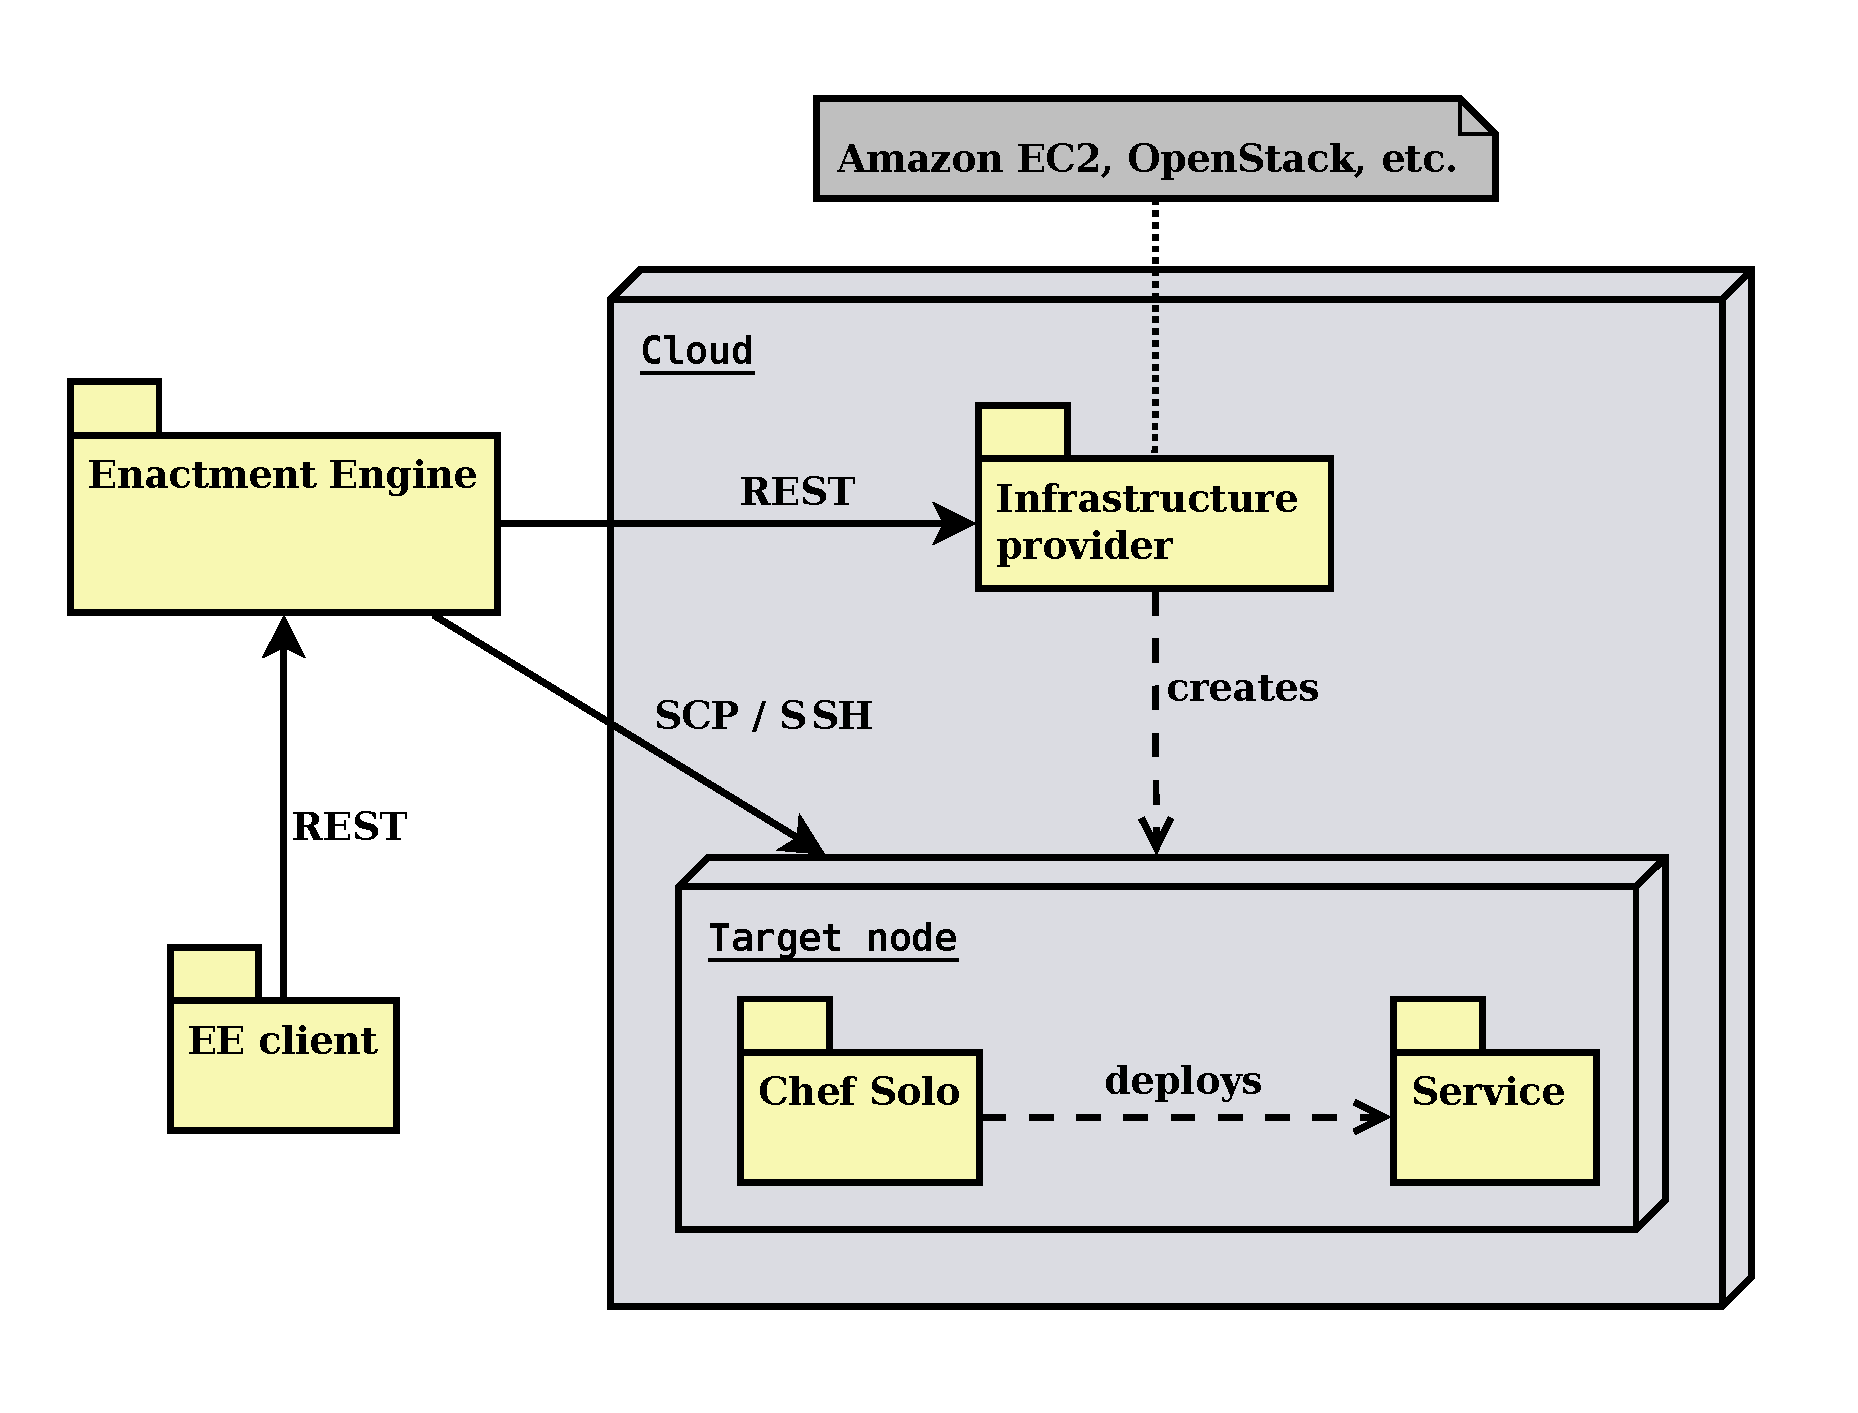
\includegraphics[scale=0.4]{img/components.pdf}
\caption{\ee\ execution environment. \todo{translate}}
\label{fig:ee_components}
\end{figure}

\begin{description}

\item [Infrastructure provider] creates and destroys virtual machines (also called \emph{nodes}) in a cloud computing environment. Currently, only Amazon EC2 and OpenStack are supported as infrastructure providers, but the \ee can be extended to support other virtualization technologies.

\item [Chef-solo] is installed by the \ee\ in each cloud node to manage ``recipes'' execution. \emph{Chef recipes} are scripts written in a Ruby-like Domain Specific Language that implement the process of configuring operational system, installing required middleware, and finally deploying the services.

\item [EE cliente] is a script, written by deployers, that specifies the choreography deployment
and invokes the EE to trigger the deployment process.
\emph{Deployer} is the human operator responsible by the deployment process. 

\item [\ee] deploys choreography services according to the specification sent by the client.

\end{description} 



\section{Requirements}

Before you run \ee, you will need:

\begin{itemize}
\item Git;
\item Java 6 or later (we are using OpenJDK);
\item Maven 3  (\url{http://maven.apache.org/download.html});
\item access to Infrastructure Provider services, as detailed in Section~\ref{sec:cloud}.
\end{itemize}

\section{Cloud Provider}
\label{sec:cloud}

A \textsf{CloudProvider} is an \ee\ interface that specifies methods to CRUD virtual machines. It is expected that a \textsf{Cloud Provider} implementations will act just as a client of some Infrastructure Provider. In this section we describe the currently available \textsf{CloudProvider} implementations and how to use them. New \textsf{CloudProvider}s may be implemented to support other virtualization tools. One example would be creating a \textsf{VirtualBoxCloudProvider} to create VMs using VirtualBox.

Whatever the cloud provider you choose, ensure that the required TCP ports of the created VMs are unblocked. Required ports: 22 to SSH, 8080, 8009, and 8005 to Tomcat, the ports used by your JAR services, and the port 8180 to EasyESB.

\subsection{Amazon EC2}

Amazon EC2 service is the simplest choice to dynamically retrieve VMs as you need. You need just to create an account at \url{http://aws.amazon.com} and configure a pair of keys to access the VMs through SSH. The trade-off is that you must pay to Amazon! 

Some hints:

\begin{itemize}
\item Request credits to education purposes: \url{http://aws.amazon.com/grants/}. The first of us earned \$500, but the others \$100. Maybe it depends on your research project description.
\item Initially there is a limit of 20 VMs that you can run simultaneously.
\item Request to increase Amazon EC2 instance limit: \url{http://aws.amazon.com/contact-us/ec2-request/}. At USP we got a 50 VMs limit.
\item If you are going to use the EC2 API directly, pay attention to the ``one-second rule'': \\ \url{http://www.a2sdeveloper.com/page-working-with-the-one-second-rule.html}. Nonetheless, \ee\ already implements the enforcement of this rule.
\item As you will be charged per hour, don't forget to shutdown/stop unused VMs.
\item You can use the Amazon EC2 web console to unblock TCP ports necessary to the choreography execution.
\item You can also use the \texttt{ec2} command line tools to manage your VMs.
\item The \ee\ creates VMs in the ``US East'' Amazon datacenter.
\item The SSH keypairs are datacenter-dependent. Therefore if you create a keypair in the EU
datacenter, it won't be valid for your VMs.
\end{itemize}

\subsection{OpenStack}

OpenStack is an open source private cloud platform that provides services to retrieve VMs as you need, in the same way that Amazon EC2. However, you must install OpenStack in your own infrastructure, which means you must own at least a little cluster (or a very powerful machine) to host the created VMs. Moreover, the OpenStack installation and configuration is not a simple task.

Some hints:

\begin{itemize}
\item OpenStack does not provide public IPs, therefore some VPN configuration is necessary to log into the provisioned nodes.
\item You can also use the \texttt{nova} command line tool to manage your VMs.
\item You need to host an Ubuntu Server 12.04 image within your OpenStack infrastructure. You will use the ID of this image to configure \ee.
\end{itemize}

\subsection{Fixed cloud provider}

If you are learning how to use the \ee\ and want just to experiment it, the \textsf{FixedCloudProvider} may be the most suitable option to you. 
It is also useful if you want to use \ee\ with your own already existing cluster machines.
With it you are responsible to manually creating and setting virtual machines and telling to \ee\ which machines must be used by it. This avoids the overhead of dealing with a cloud environment. 

When creating a virtual machine to be used by the \ee, be sure:
\begin{itemize}
\item to use the Ubuntu 12.04 as operating system;
\item it is possible to SSH into the node without typing a password: \url{http://www.integrade.org.br/ssh-without-password}\footnote{Obs: do not use a key with password.};
\item use sudo in the machine without typing a password: type \texttt{\$sudo visudo} and add the line \texttt{<user> ALL = NOPASSWD: ALL} at the end (change \texttt{<user>} by the actual user);
\item to synchronize the machine clock: \texttt{\#ntpdate ccsl.ime.usp.br};
\end{itemize}

To verify if your VM was properly set, you may run the \\ \textsf{org.ow2.choreos.deployment.nodes.cloudprovider.FixedConnectionTest} test.

The \ee\ \emph{will not} take care of bootstrapping (installing Chef) on your machines, since this process is taken only when creating new machines. 
You \emph{must} bootstrap your machines by running the \textsf{org.ow2.choreos.deployment.nodes.cm.BootstrapFixedMachines} class.
When you run the \textsf{BootstrapFixedMachines} class, \ee will bootstrap the configured fixed machines. We will talk about configuration soon.

Depending on how you create your VMs, some network configuration may be needed. In case of using VirtualBox, you can refer to \url{http://ccsl.ime.usp.br/foswiki/bin/view/Choreos/VMs}.


\section{Checkout and Compilation}

To checkout the code: \texttt{git clone https://github.com/choreos/enactment\_engine.git}. 

After installing Maven 3, open the terminal at the \texttt{enactment\_engine} folder, and run the \texttt{build.sh} script. It can take several minutes. Internet access is necessary during compilation.

\section{Configuration}

Open the folder \texttt{EnactmentEngine/src/main/resources}, and create a \texttt{ee.properties} file by copying the \texttt{ee.properties.template} file. The new properties file must be created in the same folder. Open the just created properties file and edit it following instructions on the template file. The Listing~\ref{lst:deployment_properties} shows an example. Do the same to the \texttt{clouds.properties.template} file; in the \texttt{clouds.properties} file you will define configuration to access your infrastructure provider.

\lstset{
numbers=left
}

{\footnotesize
\begin{lstlisting}[caption=ee.properties example.,label=lst:deployment_properties] 
EE_PORT=9102

# Value must be a <cloud account name> in clouds.properties
DEFAULT_CLOUD_ACCOUNT=MY_AWS_ACCOUNT

# Values in node_selector.properties
NODE_SELECTOR=LIMITED_ROUND_ROBIN

# Maximum number of VMs that can be created; set if using NODE_SELECTOR=LIMITED_ROUND_ROBIN
VM_LIMIT=10

# Creates a reservoir of extra VMs to make the deployment faster and more scalable.
# The trade-off is the cost of some more VMs.
# If the pool size reaches the threshold, the pool size is increased by one.
# To not increase your pool size, set threshold as negative or greater than the initial pool size.
RESERVOIR=true
RESERVOIR_INITIAL_SIZE=5
RESERVOIR_THRESHOLD=-1
\end{lstlisting}

\begin{lstlisting}[caption=cloud.properties example.,label=lst:deployment_properties] 
MY_CLUSTER.CLOUD_PROVIDER=FIXED
MY_CLUSTER.FIXED_VM_IPS=192.168.56.101, 192.168.56.102
MY_CLUSTER.FIXED_VM_PRIVATE_SSH_KEYS=/home/leonardo/.ssh/nopass, /home/leonardo/.ssh/nopass
MY_CLUSTER.FIXED_VM_USERS=choreos, choreos

MY_AWS_ACCOUNT.CLOUD_PROVIDER=AWS
MY_AWS_ACCOUNT.AMAZON_ACCESS_KEY_ID=SECRET
MY_AWS_ACCOUNT.AMAZON_SECRET_KEY=SECRET
MY_AWS_ACCOUNT.AMAZON_KEY_PAIR=leoflaws
MY_AWS_ACCOUNT.AMAZON_PRIVATE_SSH_KEY=/home/leonardo/.ssh/leoflaws.pem
MY_AWS_ACCOUNT.AMAZON_IMAGE_ID=us-east-1/ami-1ccc8875

MY_OPENSTACK_ACCOUNT.CLOUD_PROVIDER=OPEN_STACK
MY_OPENSTACK_ACCOUNT.OPENSTACK_KEY_PAIR=leofl
MY_OPENSTACK_ACCOUNT.OPENSTACK_PRIVATE_SSH_KEY=/home/leonardo/.ssh/nopass
MY_OPENSTACK_ACCOUNT.OPENSTACK_TENANT=CHOReOS_Sandbox
MY_OPENSTACK_ACCOUNT.OPENSTACK_USER=leofl
MY_OPENSTACK_ACCOUNT.OPENSTACK_PASSWORD=SECRET
MY_OPENSTACK_ACCOUNT.OPENSTACK_IP=http://172.15.237.10:5000/v2.0
MY_OPENSTACK_ACCOUNT.OPENSTACK_IMAGE_ID=RegionOne/1654b5b6-49b7-4039-b7b7-0e42e85480f4
\end{lstlisting}
}

The options to NODE\_SELECTOR are: 

\begin{description}
\item [ALWAYS\_CREATE:] a new VM is created to each deployed service instance.
\item [ROUND\_ROBIN:] \textsf{NodeSelector} makes a round robin using the available VMs, without creating any new VM; usually it makes sense to use it only when using the fixed cloud provider.
\item [LIMITED\_ROUND\_ROBIN:] initially the \textsf{NodeSelector} behaves like the ALWAYS\_CREATE, until a limit of created VMs is reached (VM\_LIMIT). After this limit, the selector behaves like the ROUND\_ROBIN. When using this selector, it is necessary to declare the integer VM\_LIMIT property in the configuration file.
\end{description}

The AMAZON\_IMAGE\_ID enables you to specify a customized image to be used by \ee. This feature is intended to use an image of a node already bootstrapped. In this way, the bootstrap process becomes much faster. The same may be applied to the OPENSTACK\_IMAGE\_ID. But in both cases, the image must still provide an Ubuntu Server 12.04 system.

At the \texttt{clouds.properties}, each \emph{cloud account} is configured by a group of properties grouped by a common prefix. Let's call this prefix as ``cloud account name''. These cloud account names will be compared with the \texttt{owner} attribute in the service specifications, so a service can be specified to be deployed under a specific cloud account. If there is no match, the DEFAULT\_CLOUD\_ACCOUNT value declared on \texttt{ee.properties} will be used as cloud account name.

\emph{Attention:} inline comments are not allowed in properties files. Therefore, the following would not work: \verb!VM\_LIMIT=3 \# how many instances we can afford to pay!.

\section{Execution}

After compiling the project, to run the \ee you have just to run the main method on the class \textsf{org.ow2.choreos.ee.rest.EnactmentEngineServer}.

This task can be easier accomplished if you import the \ee\ projects in the Eclipse IDE. After importing the project, open the menu \texttt{Window>>Preferences>>Java>>Build Path>>Classpath} variables, and set the \texttt{M2\_REPO} variable pointing to your Maven repository folder, usually the \texttt{.m2/repository} folder within your home folder. Obs: we have used the Eclipse Indigo version.

Another way is using maven:

\texttt{EnactmentEngine\$ mvn exec:java}

If you successfully start the EE, you must see the following message on the console: 

\texttt{\ee has started [http://localhost:9102/enactmentengine/]}

To verify if it is everything OK, run the \textsf{org.ow2.choreos.chors.SimpleChorEnactmentTest}. This test will deploy a simple choreography composed of two services and try to invoke it.


